\chapter{Introduction}
\section{Context and Motivation}
The human brain is one of the most complex and intriguing organs in the body, responsible for regulating a wide range of bodily systems and enabling us to engage in complex cognitive processes. With its billions of neurons and trillions of connections, it has captivated scientists for centuries \cite{bear2016neuroscience}.
A brain-computer interface (BCI), also referred to as a brain-machine interface (BMI), is a hardware and software communications system that enables humans to interact with their surroundings through control signals generated from electroencephalographic and  magnetoencephalographic activity. BCIs enable the translation of brain activity into commands that can be used to operate devices, such as computers or prosthetic limbs, eliminating the need of peripheral nerves and muscles \cite{wolpaw2012brain}.
BCI research is a relatively young multidisciplinary field integrating researchers from neuroscience, engineering, computer science, physiology, psychology, rehabilitation, and other technical and health-care disciplines \cite{wolpaw2012brain}.

Neural interfaces can be classified into two main categories based on the type of brain signal utilized for communication between the brain and the computer: invasive and non-invasive methods. Within these categories, there are three major classes of neural interfaces:
\begin{enumerate}
    \item Electroencephalographic (EEG) scalp electrode arrays: noninvasive attachment to the skin to record field potentials with low information content from widely distributed sets of neurons and synapses \cite{schwartz2004cortical}.
    \item Electrocorticographic (ECoG) electrode arrays: surgical positioning on the brain surface to record field potentials with moderate information content from localized sets of neurons and synapses \cite{schwartz2004cortical}.
    \item Miniaturized microelectrode arrays: surgical insertion into the cerebral cortex to record neuronal action potentials (spikes) from individual neurons and/or local field potentials (LFPs) from highly localized sets of neurons and synapses with high information content \cite{schwartz2004cortical}.    
\end{enumerate}

Non-invasive measurement techniques include functional magnetic resonance imaging (fMRI) \cite{glover2011overview}, functional near-infrared spectroscopy (fNIRS) \cite{chen2020functional}, magnetoencephalography (MEG) \cite{singh2014magnetoencephalography} and electroencephalography.
EEG is a non-invasive technique used to measure the electrical activity of the brain. EEG works by recording the electrical signals in the brain that are related to the flow of electric currents during synaptic excitation of neuronal dendrites, especially in the cortex, but also in the deep brain structures \cite{nicolasalonso2012brain} using electrodes placed on the scalp. These signals are amplified and processed to create a visual representation of the brain's activity, known as an EEG waveform or EEG trace \cite{bear2016neuroscience}. EEG-based BCI systems can be dated back to 1971, when a prosthetic arm was developed and could be controlled by EEG \cite{nirenberg1971new}. Since then, EEG has been widely studied to develop BCIs for controlling and communication \cite{birbaumer2007brain}.

The EEG waveform is characterized by different frequency bands, including delta ($<$ 4 Hz), theta (4-7 Hz), alpha (8-12 Hz), beta (12-30 Hz), and gamma waves (30-100 Hz). Each frequency band corresponds to a different level of brain activity, with delta waves representing deep sleep or unconsciousness, and gamma waves representing high-level cognitive processing \cite{schwartz2004cortical}.

EEG has several advantages over other brain imaging techniques, including its portability, low cost, high temporal resolution, and ability to measure brain activity in real-time \cite{niedermeyer2005electroencephalography}. However, it also has some limitations, such as its relatively low spatial resolution compared to techniques like fMRI and positron emission tomography (PET) \cite{luck2014introduction}.

Despite its limitations, EEG remains a valuable tool for studying the brain and has led to significant advances in our understanding of brain function. Ongoing research is focused on developing new EEG-based techniques for clinical diagnosis and treatment, as well as for cognitive enhancement and brain-computer interfaces \cite{mullerputz2005steadystate}.

Before diving into visual-based BCIs, it is important to understand some key performance metrics used to evaluate and compare different BCI systems. These metrics include accuracy, information transfer rate (ITR), signal-to-noise ratio (SNR), and user training requirements \cite{wolpaw2002brain}. Accuracy refers to the system's ability to correctly identify the user's intended command, while ITR measures the amount of information transmitted per unit of time, usually expressed in bits per minute (bpm). SNR represents the quality of the brain signal extracted by the BCI system, with a higher SNR indicating better signal quality and improved performance. Lastly, user training requirements reflect the ease of use and adaptability of a BCI system, with lower training requirements being more desirable for efficient and user-friendly interfaces \cite{kubler2007introduction}.

\begin{figure}
    \centering
    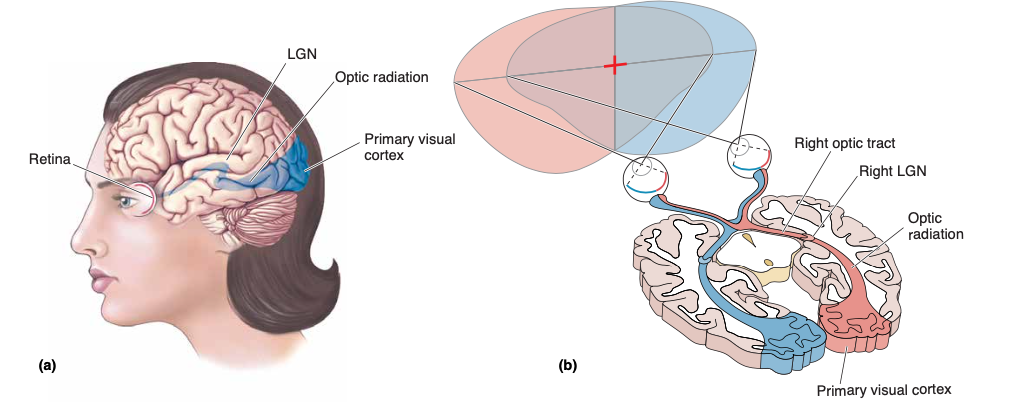
\includegraphics[width=0.75\textwidth]{images/intro/visual pathways.png}
    \caption{The visual pathway that mediates conscious visual perception. (a) A side view of the brain with the retinogeniculocortical pathway shown inside (blue). (b) A horizontal section through the brain exposing the same pathway(adapted from \cite{bear2016neuroscience}).}
    \label{fig:visual}
\end{figure}

To understand the foundation of visual-based BCIs, it's crucial to comprehend the basic visual pathway in humans which is shown in Figure \ref{fig:visual}. Light enters the eye through the cornea and is focused onto the retina, where it stimulates photoreceptor cells. These cells convert light into electrical signals, which are transmitted to the brain via the optic nerve. These signals first pass through the optic chiasm, where the information from the left and right visual fields are segregated. These segregated signals then travel through the lateral geniculate nucleus of the thalamus, where they are processed and sent to the primary visual cortex. This complex pathway allows for the detailed and nuanced visual processing that underlies our visual perception \cite{bear2016neuroscience}.

Building on the complexity of the visual pathway in humans, another intriguing aspect is the phenomenon of binocular vision and binocular rivalry. Binocular vision refers to the ability to integrate visual information from both eyes, providing depth perception and a more comprehensive view. Binocular rivalry, a subject of intensive investigation for over 160 years, occurs when dissimilar images are presented to corresponding regions of the two eyes. Rather than merging into a single view, the two images compete for perceptual dominance, with one image dominating conscious awareness for several seconds before being supplanted by the previously suppressed rival image. This rivalry reveals important grouping properties and provides a powerful tool for studying the neural concomitants of conscious visual awareness. The most recent evidence supports a view of rivalry as a series of processes, each implemented by neural mechanisms at different levels of the visual hierarchy, indicating the operation of nonlinear dynamical processes. This concept is foundational to understanding how the brain processes conflicting visual information and has implications for visual-based BCI systems \cite{blake2002visual}.

Visual-based BCI systems are a subset of brain-computer interfaces that specifically focus on utilizing the brain's visual processing capabilities to control external devices or communicate with the environment \cite{allison2007brain}. These systems often rely on the detection and interpretation of brain signals generated in response to visual stimuli, such as patterns, images, or flickering lights \cite{mullerputz2005steadystate}. As a result, visual-based BCIs can provide a more intuitive and user-friendly experience, allowing individuals to interact with their surroundings using natural visual attention and perception processes \cite{cecotti2011spelling}. Researchers continue to explore novel visual-based BCI paradigms to enhance system performance and usability, with the goal of developing practical applications for individuals with various needs, such as those with limited mobility or communication challenges \cite{guger2009many}.

The P300 paradigm, along with code-modulated visual evoked potentials (c-VEP) and transient visual evoked potentials (t-VEP), represents another approach in the field of visual-based BCIs \cite{wolpaw2012brain}. P300 is an event-related potential (ERP) characterized by a positive deflection in the EEG signal, typically occurring around 300 milliseconds after the presentation of a rare or unexpected stimulus \cite{sutton1965evoked}. Both c-VEP and t-VEP paradigms exploit the brain's response to specific visual stimuli, with c-VEP focusing on the rapid presentation of pseudorandom sequences \cite{sutter1992brain} and t-VEP capturing responses to sudden changes in the visual scene \cite{bin2009online}. While these methods have shown potential in BCI applications, the focus remains on the SSVEP paradigm.

SSVEP is a periodic brain electrical response induced by the repetitive presentation of a visual stimulus, flickering or reversing at a certain frequency ranging from 1 Hz to 60 Hz \cite{zhu2010survey}. The SSVEP-based BCI has many advantages over other BCI systems, including a higher SNR and ITR. Also, since the SSVEP is an inherent response of the brain, very little training is required to enable a person to operate the BCI \cite{bakardjian2010optimization}.

Although SSVEP can be elicited by a broad range of frequencies, the available frequencies in practical BCI applications are often restricted by several factors. First, all available stimulation frequencies do not always evoke high SSVEP responses. The frequencies that elicit strong SSVEP responses are highly dependent upon the participants, as well as various properties of the visual stimuli, such as color, size, and contrast \cite{zhu2010survey}. Second, the use of two frequencies, $f_1$ and $f_2$, in the same experiment has been typically avoided when $f_1$ is a multiple of $f_2$ or vice versa because of the harmonic SSVEP responses \cite{cheng2002design,shyu2010development,wang2017benchmark}.
\begin{figure}
    \centering
    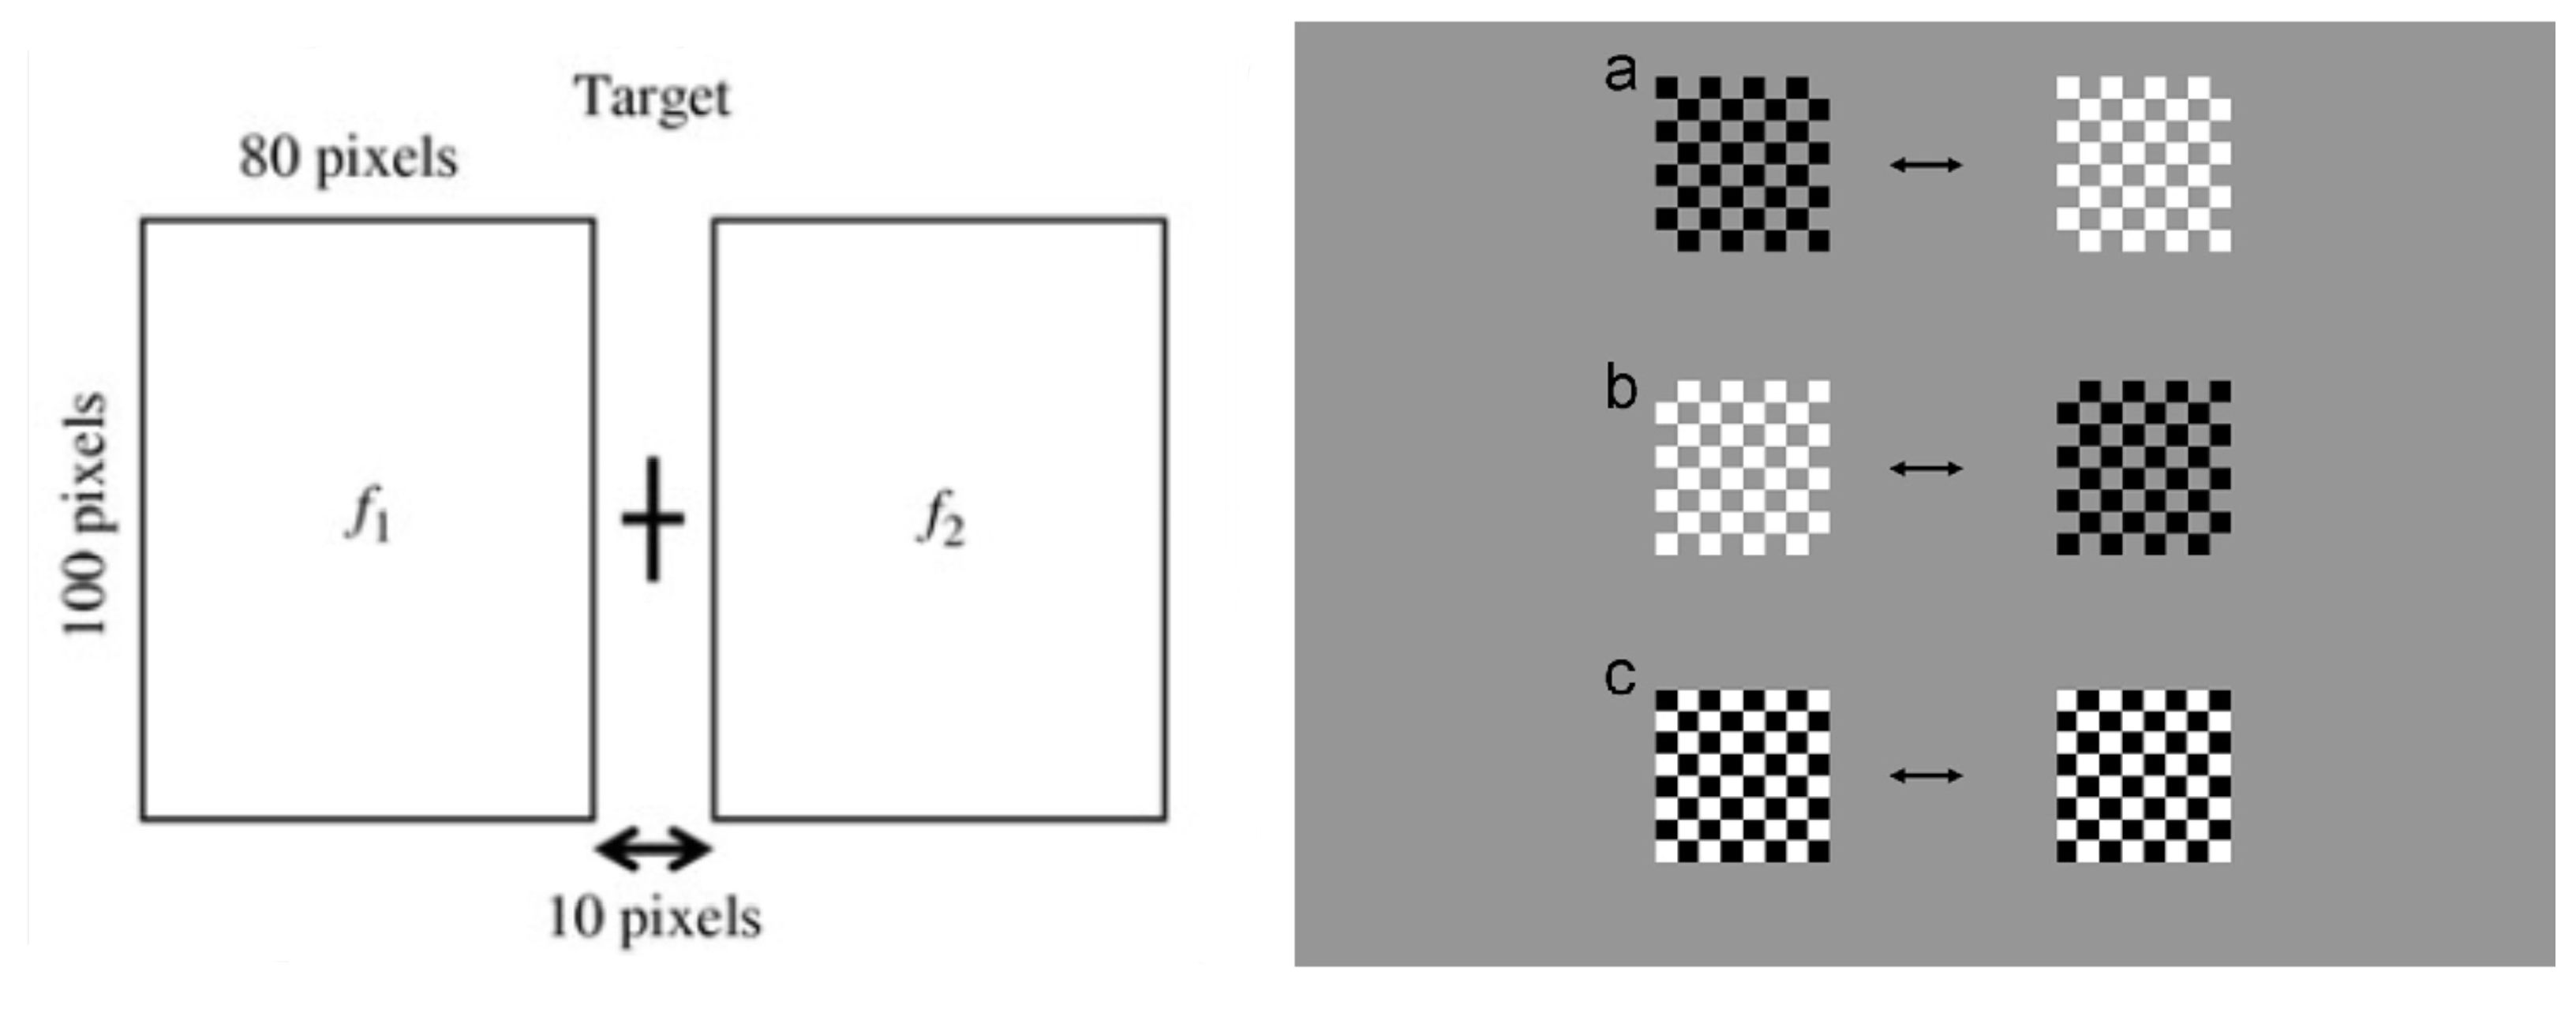
\includegraphics[width=0.75\textwidth]{images/intro/dual.png}
    \caption{Composite image showing the left-right view paradigm (adapted from \cite{yan2011right}) and the checkerboard paradigm (adapted from \cite{hwang2013new}).}
    \label{fig:dual}
\end{figure}
Dual-SSVEP paradigms have been developed to address some of the limitations of single-frequency SSVEP systems. In a dual-SSVEP paradigm, two different frequencies, $f_1$ and $f_2$, are simultaneously presented to the user, typically using one of two methods: the left-right view paradigm or the checkerboard paradigm \cite{vialatte2010steadystate,mullerputz2008control}. Figure \ref{fig:dual} illustrates these two paradigms, with the left-right view paradigm shown on the left and the checkerboard paradigm on the right.

In the left-right view paradigm, each frequency is presented in a distinct spatial location, usually with $f_1$ in the left visual field and $f_2$ in the right visual field. The user can select one of the multiple targets by focusing their attention on the fixation point. This approach does not merely double the number of available targets, as initially suggested, but actually increases the number of potential targets combinatorially. Given $n$ different frequencies, the number of potential targets is of the form $C_{n2}$ (combinations of $n$), since two frequencies can be used simultaneously \cite{mullerputz2008control,zhang2015toward,min2014neuroimaging,friman2009spelling}. Furthermore, this paradigm enhances the robustness of the BCI by reducing the impact of transient attentional shifts and visual fatigue, which can affect the performance of single-frequency SSVEP systems \cite{mullerputz2008control,zhang2015toward,min2014neuroimaging,lin2007frequency}.

The checkerboard paradigm, on the other hand, involves presenting the two target frequencies as alternating squares in a checkerboard pattern. This arrangement allows the user to focus on the entire visual field, and the response of the brain to the target frequencies can be selectively attended to and decoded by the BCI system \cite{min2014neuroimaging,cao2020highperformance,chen2015filter}. The checkerboard paradigm has been shown to improve the stability of the SSVEP response and increase the ITR compared to the left-right view paradigm \cite{min2014neuroimaging,cao2020highperformance,pan2011detecting}.

Overall, both the left-right view and checkerboard paradigms offer advantages over single-frequency SSVEP systems. They increase the number of control commands without increasing the visual complexity of the interface, making them more attractive for practical applications \cite{lin2017frequency,mullerputz2005steadystate}. Moreover, by exploiting the brains natural ability to selectively attend to different visual stimuli, dual-SSVEP paradigms can provide a more intuitive and user-friendly BCI experience \cite{trenado2019enhancing,bin2011vepbased}.

Despite its potential advantages, dual-SSVEP systems still face some challenges \cite{cheng2002design,shyu2010development,wang2017benchmark}. One major issue faced by dual-SSVEP systems is the unpredictable intermodulation (IM) of the harmonic components \cite{sun2023binocular}. Intermodulation components arise when different elements of a stimulus are modulated using more than one frequency, leading to neural responses not only at the original frequencies but also at additional frequencies. These IM components result from the non-linear integration of neural signals driven by differentially modulated stimulus elements. IM components have been used in frequency tagging neuroimaging designs and have emerged as a promising direct measure of neural interactions. They have initially been used to investigate low-level visual processing and are now being applied to study mid- and high-level perceptual processes, including the involvement of cognitive functions such as attention and expectation. IM components provide direct evidence for non-linear interactions within the visual pathways and offer insights into the existence, degree, and type of neural integration mechanisms at hand \cite{gordon_intermodulation_2019}.

\section{Problem Statement}

In recent years, research into BCIs has gained significant interest as a means of providing communication and control for individuals who have lost the ability to move or speak due to neurological disorders or injuries. One promising type of BCI is the SSVEP, which utilizes the brain's response to visual stimuli presented at specific frequencies to communicate information. However, conventional dual-SSVEP paradigms have certain shortcomings, such as intermodulation of harmonic components, which can lead to reduced accuracy and reliability of the SSVEP response.

To address these shortcomings, a novel binocular dual-SSVEP paradigm in a polarized display system was recently proposed \cite{sun2023binocular}, according to which, Information Transfer Rate (ITR) can be increased, and noise can be reduced compared with traditional dual-SSVEP paradigms. However, the polarized-light system used in the study is rather impractical to use in daily life. Therefore, the present study aims to evaluate a novel dual-SSVEP paradigm using virtual reality (VR) technology. VR has several benefits for BCI applications, such as the ability to control what each eye sees individually, providing more control of what the user sees and greater immersion. By utilizing VR to present the SSVEP stimuli to each eye separately, it may be possible to remove the IM of harmonic components and improve the accuracy and reliability of the SSVEP response.

The goal of this thesis is to evaluate the feasibility and effectiveness of this new dual-SSVEP paradigm in a VR environment. The specific objectives are to design and implement a VR-based dual-SSVEP paradigm, evaluate the paradigm's performance in terms of accuracy and reliability of the SSVEP response using the power spectral density (PSD) as a metric, and compare the performance of the VR-based dual-SSVEP paradigm to that of a conventional dual-SSVEP paradigm.

\subsection{Research Questions}

Building on the identified limitations of conventional dual-SSVEP paradigms, this study aims to explore the efficacy of a VR-based approach in enhancing the accuracy and reliability of SSVEP responses.
The research is guided by several key questions, as outlined in Table \ref{tab:comparisons} below. Overall, the proposed study has the potential to significantly advance the development of SSVEP-based BCIs by addressing the shortcomings of conventional dual-SSVEP paradigms and improving the accuracy and reliability of the SSVEP response. By utilizing VR technology, the study may also provide new insights into the neural mechanisms underlying SSVEP responses and the role of visual processing in BCI applications.

\begin{landscape}
    \begin{table}
    \centering
    \begin{tabularx}{\linewidth}{>{\centering\arraybackslash}p{0.75cm}>{\centering\arraybackslash}p{3.5cm}>{\raggedright\arraybackslash}X>{\raggedright\arraybackslash}X}
        \hline
        
        \textbf{Exp.} & \textbf{Conditions} & \textbf{Research Question} & \textbf{Null Hypothesis} \\
        
        \hline
        \addlinespace
        1 & L$f_{1}$R$\varnothing$ vs. L$f_{1}$R$f_{1}$ vs. L$\varnothing$R$f_{1}$ & 
        Can we differentiate hemisphere-specific SSVEP responses based on the visually stimulated eye? & There is no difference in SSVEP responses or hemisphere-specific activity regardless of which eye is stimulated. \\
        \addlinespace
        \addlinespace
        \addlinespace
        2 & L$f_{1}$R$f_{2}$ vs. L$f_{2}$R$f_{1}$ & 
        Can we differentiate SSVEP responses based on the unique frequency stimuli presented to each eye? & SSVEP responses cannot be differentiated based on the unique frequency stimuli presented to each eye. \\ 
        \addlinespace
        & & Can we simultaneously elicit separate SSVEP responses in both hemispheres? & Separate SSVEP responses cannot be simultaneously elicited in both hemispheres. \\
        \addlinespace
        4 & \makecell{(FL - BR L$f_{2}$,~R$f_{1}$)\\vs.\\(FR - BR L$f_{2}$,~R$f_{1}$)} & Can the direction of participants' attention control or influence binocular rivalry? & The direction of participants' attention has no control or influence over binocular rivalry. \\
        \addlinespace
        \hline
    \end{tabularx}
    \caption{Overview of the experimental comparisons and the associated research questions.}
    \emph{Note: In the notation, L$f_{1}$R$\varnothing$ represents the left eye seeing frequency $f_{1}$ and the right eye seeing no stimulation (absence denoted by "$\varnothing$"). Similarly, L$f_{2}$R$f_{1}$ represents the left eye seeing frequency $f_{2}$, and the right eye seeing frequency $f_{1}$. \\
    BR = Binocular Rivalry; FL/FR = Focus Left/Right}
    \label{tab:comparisons}
\end{table}
\end{landscape}

\section{Literature Review}

SSVEPs driven BCIs are a significant area of research. The focus of this literature review is on the challenges and advancements in dual-frequency SSVEPs, particularly in the context of the proposed novel dual-SSVEP paradigm using VR technology.

Hwang et al. \cite{hwang2013new} introduced a novel dual-frequency stimulation method to increase the number of visual stimuli for multi-class SSVEP-based BCIs. This approach overcame the "attention-shift" problem by using a single visual stimulus mixed with two different patterns. The method utilized a conventional black-white checkerboard pattern and generated ten visual stimuli by combining four different stimulation frequencies. The implementation of a mental keypad system using this method reported an average information transfer rate of 33.26 bits/min and an average accuracy of 87.23\%. The hypothesis of this paper was that the dual-frequency stimulation method could enhance the number of visual stimuli without increasing complexity. The study also highlighted the importance of the selection of stimulation frequencies and the design of visual stimuli, which are directly related to the aim of the current study.

Chen et al. \cite{chen2015filter} developed a filter bank canonical correlation analysis (FBCCA) method to enhance SSVEP detection. The paper introduced three methods (M1, M2, M3) for optimizing filter bank design, each with different sub-band decompositions. The FBCCA methods were compared with the standard CCA method for classification accuracy and ITR. Method M3 achieved the highest classification performance, and an online BCI speller using the optimal FBCCA method achieved an average ITR of \(151.18 \pm 20.34\) bits min\(^{-1}\). The assumption in this paper was that incorporating fundamental and harmonic SSVEP components would improve detection. The study also discussed the importance of the spatial filter design and the need for individual calibration, aligning with the focus of the current study on improving accuracy and reliability.

Yan et al. \cite{yan2011right} proposed a right-and-left visual field stimulation technique where each visual stimulus was characterized by a spatial frequency and a temporal frequency. This approach significantly increased the number of possible commands without increasing the number of visual stimuli. The paper identified challenges such as the complexity of visual stimuli and the likelihood of IM components. The hypothesis of this paper was that a right-and-left visual field stimulation technique could enhance command possibilities without increasing stimuli. The study also explored the use of different algorithms for frequency recognition and the potential for user-specific customization, providing insights into the focus of this current study on novel dual-SSVEP paradigms.

Sun et al. \cite{sun2023binocular} introduced a novel binocular dual-SSVEP  paradigm utilizing a polarized display system. The primary objective of their research was to enhance the ITR and minimize noise, thereby improving upon traditional dual-SSVEP paradigms. Their hypothesis posited that a binocular approach could significantly improve ITR while reducing noise, although they acknowledged the current technological limitations as a constraint. 

The study is particularly noteworthy for its comprehensive experimental design, which included two key experiments. The first, a 6-target offline experiment, demonstrated a 2 dB increase in the SNR of target frequency components when compared to unpredictable IM components. This result indicates a more stable and reliable signal, which is crucial for the practical application of BCI. The second experiment was an online 40-target test that yielded an average ITR of \(104.56 \pm 15.74\) bits/min. Remarkably, this rate is nearly double that of existing dual-frequency paradigms, underscoring the efficacy of their novel approach.

Furthermore, Sun et al. contributed to the algorithmic aspect by introducing an improved filter bank dual-frequency canonical correlation analysis (FBDCCA). This algorithm is tailored for dual-frequency SSVEP paradigms and serves to further optimize the system's performance. In addition to these technical contributions, the paper also delved into the spatial separation of visual stimuli and explored the potential for integrating other sensory modalities. While the study is a significant step forward, it also highlights the impracticality of the current technology as a limitation. The current research aims to evaluate a similar dual-SSVEP paradigm but leverages Virtual Reality technology, potentially overcoming some of these limitations.
